%% We use `subfiles' package
\documentclass[preamble.tex]{subfiles}
\begin{document}

\pagebreak{}

\section{Loop representation: The Loop Language}

LiveFusion at the top level presents a library of high level array combinators, with each one representing a particualar array operation. Many of them conceptually represent a loop. However, we would like to be able to perform several such operations in one loop, whenever possible. Such fusible loops arise in the case where the result of one combinator is consumed as input by another. In the LiveFusion AST constructed at runtime this would correspond to a child producer node and its parent consumer node. How do we know whether two combinators can be fused? We discussed in Section (TODO ref) that just it is impractical for libraries with a large number of combinators to define rewrite rules for how each potential pair of combinators is fused together. We need to be more general than that. In principle, two combinators can be fused whenever you can write a loop by hand which would give the same result for the same input. We need a way to programmatically determine whether a given pair of combinators can be replace with a semantically equivalent loop.

The focus of this chapter is to establish the requirements for fusible combinators and define a loop representation to which such fusible combinators can be mapped.



%% \subsection{Nature of fast loops}

%% + inherently procedural
%% + several combinators fuse to a single loop
%% + must generate parts of the same loop



\subsection{Anatomy of a loop}

Despite the purely functional, combinatorial interface to the library, looking at a loop in a purely procedural way is the approach we opted for in the middle layer. It is represented by the Loop language. The loops we generate can be viewed as similar to those in the mainsteam procedural languages such as C, however there are two important differences. One positions our Loop language a step above the simple C loops while the other one, sadly, is what C programers are trying to avoid.

On the positive side, we offer a language that logically separates sections of a loop such as initialisation, body and update. It makes it more clear which variables carry mutable state of the loop and which are immutable.

The downside, however, is that our loop relies on \|goto|-like statements whose use is almost always considered bad practice in modern software engineering.

Without further delaying the discussion of the matter we will now look are the stucture of a typical loop and gradually extend it to what we need.

Let us take a simple function which adjusts elements of an array by applying a certain function $f$ and then picks out elements which are above a certain threshold, say 100. In Haskell the function would have looked something like the following:

\begin{figure}
\begin{subfigure}{.7\textwidth}
  \begin{hscode}
  aboveThreshold :: (Double -> Double)
                 -> Array Double
                 -> Array Double
  aboveThreshold xs f
    = let adjusted = map f xs
          above    = filter (> 100) adjusted
      in  above
  \end{hscode}
\end{subfigure}%
\begin{subfigure}{.3\textwidth}
  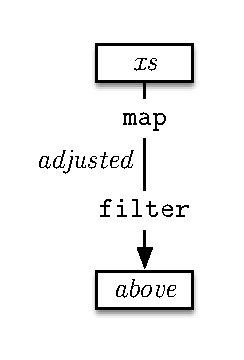
\includegraphics[height=12em]{img/aboveThreshold}
\end{subfigure}
\caption{$aboveThreshold$ function (left) and its data flow (right).}
\label{fig:Loops:aboveThreshold}
\end{figure}

We will now present a corresponding C solution and try to pull it apart into its constituent parts. This is not canonical code most C programmers would write. However, it does, like the Haskell example above, run each combinator in a separate loop and allocates all intermediate arrays\footnote{Function pointer syntax is not one of C's strengths, so we omitted it from the list of arguments}.

\begin{ccode}{numbers=left}
double* aboveThreshold (double xs[], int len, int *result_len ) {

  /* Adjust all values by mapping function f over each element */
  double* adjusted = malloc(len * sizeof(double)); // Intermediate array
  for(int i=0; i<len; i++) {
      adjusted[i] = f(xs[i]);
  }

  double* above = malloc(len * sizeof(double));     // Final result array
  int o = 0; // result array index
  for(int i=0; i<len; i++) {
      double a = adjusted[i];
      if(a > 100) {
          above[j] = a;
          o++;
      }
  }
  above = realloc(above, o * sizeof(double));
  free(adjusted);

  // return results
  *result_len = o
  return above;
}
\end{ccode}


\subsubsubsection{Sections of \|for|-loop}
Each \|for|-loop in C has four sections: \|initialisation| ($i=0$), \|guard| ($i<len$), the main \|body| and finally, the \|update| section ($++i$). Compared to free-formed \|while|-loops which only have the \|guard| and the \|body|, the \|for|-loops are already more stuctured. However, as we will now show, futher structural elements could be introduced to assist fusion.

\subsubsubsection{Initialisation}
The very first observation to make is that the allocation of intermediate and result arrays was done by statements outside the \|for|-loops. The same was done for the output index variable $o$ (which is different from input index $i$ because \|filter| can skip elements). In our loop language all statements executed *once* before the loop begins are placed in the \|init| block of the loop.

The \|init|-code for both loops would have looked like the following (we also included \|guard| code for clarity):
\begin{loopcode}
  init_1:
    len_1 = arrayLength xs
    adjusted_1 = newArray len_1
    i_1 = 0
    goto guard_1

  guard_1:
    guard (i_1 < len_1) done_1
    goto body_1

  init_2:
    len_2 = arrayLength adjusted_1
    i_2 = 0
    o_2 = 0
    goto guard_2

  guard_2
    guard (i_2 < len_2) done_2
    goto body_2

\end{loopcode}

As we will soon see the above code is only illustrative. Even though it is valid, the combinators in the $aboveThreshold$ example do not generate precisely that code.

\subsubsubsection{Finalisation}
We also note that after the second \|for|-loop finishes, the resulting array is reallocated to free the unused memory since the filter results in a shorter array in the general case (in practice the array is unlikely to be copied). This is one of the use cases for what we call a \|done| block, which every array has. As we will see later it is not only useful for trimming and returning the final array but also for scheduling other loops such as in $append$ combinator.

The done blocks for the arrays would look like the following:

\begin{loopcode}
  done_1:
    <empty>

  done_2:
    above := freezeArray above o  -- resize to length `o'
\end{loopcode}

\subsubsubsection{Reading and writing arrays}
We will now attempt to categorise the types of operations that all belong to the bodies of conventional \|for| and \|while| loops.

Line 5 of the first \|for|-loop (\inlc{adjusted[i] = f(xs[i]);})is actually doing three things: *reading* an element from an array, *producing* a new element and *writing* it into a separate array. Likewise, Lines 12 and 14 of the second \|for|-loop are also concerned with *reading* and *writing* arrays.

Consider, however, that when several combinators are fused into a sigle loop and produce no intermediate arrays, such reading and writing only happens at the beginning and at the end of a combinator pipeline. Thus we want to separate the notion of computing a new element from from the fact that it came from an array, a list or just another computation. Likewise we do not need to be concerned with whether the how the new element is going to be consumed. It may or may not be written into a new array. However, it is not up to an individual combinator to decide.

We will now in turn describe how we deal with reading, writing and computing elements.

\subsubsubsubsection{Reading and writing arrays in LiveFusion}
It is now time to remember the \|Manifest| combinator of LiveFusion language that we used to bring a physical array in memory and create a LiveFusion language term out of it. As it turns out, \thesis{all the reading of physical arrays is performed by the code generated by the \|Manifest| combinator}. What this means is that, while the reading is still performed in the \|body| code block of of the loop, the code for it is only generated once at the beginning of each combinator pipeline.

Applied to the function from our $aboveThreshold$ example, this tells us that since we don't know which combinator produced the $xs$ array, the loop code generated for the $aboveThreshold$ function will *not* inlcude the specifics of where the individual elements of $xs$ came from.

\begin{loopcode}
  -- Loop: $adjusted$ = \|map| $f$ $xs$
  init_adj:
    goto guard_adj

  guard_adj:
    goto body_adj

  body_adj:
    elt_adj = f elt_xs
    goto yield_adj

  yield_adj:
    goto bottom_adj

  bottom_adj:
    goto guard_adj

  done_adj:


  -- Loop: $above$ = \|filter| $(>100)$ $adjusted$
  init_abv:
    o_abv = 0
    goto guard_abv

  guard_abv:
    goto body_abv

  body_abv:
    elt_abv = elt_adj
    guard (elt_abv > 100) bottom_abv
    goto yield_abv

  yield_abv:
    o_abv := o_abv + 1
    goto bottom_abv

  bottom_abv:
    goto guard_abv
\end{loopcode}

One will immediately notice the absence of loop counters $i$, array read/writes or allocations. Instead we only see some references to undeclared variables $elt_xs$, $elt_adj$, $elt_abv$. These represent the values of elements of $xs$, $adjusted$ and $above$ arrays at each iteration\footnote{In our implementation all variables, block labels and AST/ASG nodes are given a unique label, an integer. For readability we replaced those with meaningful subscripts.}

It is clear that these two loops are incomplete and cannot be run by themselves. Now suppose that the function $aboveThreshold$ is actually applied to some manifest array $xs$ (where $xs$ is a Vector in current implementation) and that the result of this application is forced to a manifest array, for example:
% Perhaps the manifest array should be stored with the node in an IORef/M
\begin{hscode}
let accepted = aboveThreshold abs (Manifest xs)
in  ...random access $accepted$...
\end{hscode}

What happens is that two new loops are generated: one for \|Manifest| $xs$ and one for the physical array creation:

\begin{loopcode}
  -- Loop: \|Manifest| $xs$
  init_xs:
    len_xs = arrayLength xs
    i_xs = 0
    goto guard_xs

  guard_xs:
    guard (i_xs < len_xs) done_xs
    goto body_xs

  body_xs:
    elt_xs = readArray xs i_xs
    goto yield_xs

  yield_xs:
    goto bottom_xs

  bottom_xs:
    i_xs := i_xs
    goto guard_xs

  done_xs:


  -- Loop: forcing $aboveThreshold f xs$
  init_force:
    result = newArray len_xs
    goto guard_force

  guard_force:
    goto body_force

  body_force:
    goto yield_force

  yield_force:
    writeArray result o_abv elt_abv
    goto bottom_force

  bottom_force:
    goto guard_force

  done_force:
    result := freezeArray result o
\end{loopcode}

The \|Manifest| loop is the only one of the four ``loops'' presented so far that actually resembles a runnable loop. Out of the four it is the only one that introduces a source array counter $i_{xs}$ in the \|init| block which it compares against the length of $xs$ in the \|guard|. It also increments it in the \|bottom| block.

All in all the \|init|, \|guard| and \|bottom| blocks of the \|Manifest| $xs$ loop resemble very closely the \|initialisation|, \|guard| and \|update| section of the \|for| loops we presented earlier in our C version of the function. We will revisit this comparison very soon.

We have essentially given the complete Loop representation for \|Manifest|, \|map| and \|filter| combinators together with the code that actually deals with writing out physical arrays. However, it all came in separate loops none of which was very useful by itself. We will now show how these loops can be turned into a runnable loop.

\subsubsubsubsection{Merging loops}

In the previous section we have established how each of the combinators of the $aboveThreshold$ function contribute to each loop. Each of those loops has \|init|, \|guard|, \|body|, \|yield|, \|bottom| and \|done| code blocks which are connected by \|goto|s. We can now simpy merge the respective sections of all loops to give a loop in Figure . The statements of \|Manifest| array itteration preceed those of the \|map|, which in turn preceed those of the \|filter|. The statements of physical array creation come last.

\begin{loopcode2}{Final loop for a call of $aboveThreshold$ Function}{Fig:Loop:aboveThreshold-final-loop}
  -- Loop: force \$ filter (> 100) \$ map f \$ Manifest xs
  init:
    len_xs = arrayLength xs          -- From \|Manifest|
    i_xs = 0                         -- From \|Manifest|
    o_abv = 0                        -- From \|filter|
    result = newArray len_xs         -- From forcing result
    goto guard

  guard:
    guard (i_xs < len_xs) done       -- From \|Manifest|
    goto body

  body:
    elt_xs = readArray xs i_xs       -- From \|Manifest|
    elt_adj = f elt_xs               -- From \|map|
    elt_abv = elt_adj                -- From \|filter|     
    guard (elt_abv > 100) bottom     -- From \|filter|
    goto yield

  yield:
    o_abv := o_abv + 1               -- From \|filter|
    writeArray result o_abv elt_abv  -- From forcing the result
    goto bottom

  bottom:
    i_xs := i_xs                     -- From \|Manifest|
    goto guard

  done:
    result := freezeArray result o   -- From forcing result

\end{loopcode2}

Talk about loop merging........

An important difference however, is that while in the C version there were two separate loops with separate counters ...



% section more_on_ (end)
+ Init
+ Guard
+ Body
+ Bottom
+ Done
+ Proceed by showing an exaple, slowly populating the loop
+ Identify problem of identifying common variables
+ Identify the problem of naming conventions

\subsubsection{More on \texttt{goto}'s}

While the use of \texttt{goto}'s is considered bad practive in modern software engineering we note several reasons for using them in our intermediate language:
+ It is completely hidden from the library user. Given a well behaving Loop code generator the produced code will always be valid if the user program is valid. This is akin to using \|unsafePerformIO| and similar combinators within the guts of the library for performance reasons. They can lead to bad code but with careful use give very noticeable advantages to purely functional programs.
+ The library was designed with pluggable backend in mind. It was assumed that assembly-like Loop language would be easier to connect with any backend. Specifically for Haskell backend, \|goto| statements are translated to tail-recursive function calls.
+ The \|goto|-based design seemed to be the most flexible and the easiest to implement. None-the-less, the Loop language may be extended to support a safer and more advanced implementation where individual *blocks* become functions.


\subsubsection{Block names}


+ Many of the combinators use a similar set of variables, e.g. both Map and Scan produce a value at each iteration which they assign to an intermediate variable in the body of the loop, say elt
+ Thus if there are two maps one after the other, we need to distinguish between the two
+ We give earch such variable a unique identifier which coincides with the identifier of the combinator in the graph (see section), e.g. $elt_3$ is always an intermediate element produced by combinator 3 in each iteration (provided the combinator is a producer)
+ Other examples include $len_3$, $len_1$, $i_1$, $o_5$, $acc_4$
+ Not only this removes any potential name clashes (since ids are unique), but also allows us to refer to any variable in the loop just knowing what function it's performing as well as the combinator id.
+ When is it useful? Can we have a DS passing those variables without stupid conventions?
+ The problem is that the names are generated by convention, so in case of any error, the program would either fail to compile at runtime or produce incorrect results
+ The easiest way 
+ Like global variables
+ Spooky action at a distance
+ Untracked interaction between different parts of loop
+ In many cases a flaw of software design, often discouraged and even semantically prohibited in functional languages like haskell and ml.



\subsection{Communication by Convention}

We have discussed that our loop clauses are being populated by combinators that do not know how many other combinators are in the pipeline or what these combinators are. And yet, once all of the combinators have filled in their parts, we end up with just one loop in which those combinators operate on the shared state. We will now discuss the approach by which those combinators cooperate with each other inside a single loop and how the state produced by one combinator is passed on to the combinators in the subsequent parts of the pipeline.

Let's look a simple example of what shared state a pipleline of two combinators \inlc{map g \$ map f \$ xs} is.


\subsubsection{\label{sec:Loop:Elts}Intermediate values}

As usual we decompose each combinator into a set of loop clauses. We have done this for the \|map| combinator in the previous section. However, the added complication is that there are two \|map|s, both of which expect an input value in $elt_i$ and and produce an output value in $elt_o$ at each iteration. This results in variable name clashes. We could give them unique names $elt_{i_1}$, $elt_{o_1}$, $elt_{i_2}$ and $elt_{o_2}$ based on the number of the combinator in the pipeline. We also notice that the output $elt_{o_1}$ of \|map f| is fed as input $elt_{i_2}$ to \|map g|. A simple solution is to introduce an equation $elt_{i_2} = elt_{o_1}$ for each combinator. This is the first example of interaction between combinators through shared state.
 $elt_{i_2} = elt_{i_1}$ might not be terribly exciting to read about

In the above example, we have established that for combinators that consume one element in each iteration, such as \|map|, \|fold| or \|filter|, that element would be stored in variable $elt_{o_n}$ where *n* is the the unique number of the previous combinator in the pipleline. The prefix $elt_o$ is its generic form and designates the intermediate output value in an iteration. This is the first *convention* that we use in our *Loop* language to tie together the code generated by different combinators.

The two combinators |map g . map f| give us code similar to the following:

\begin{lstlisting}[mathescape]
body:
  $elt_{i_1}$ = $elt_{o_0}$          -- input  of `map f'
  $elt_{o_1}$ = f $elt_{i_1}$  -- output of `map f'
  $elt_{i_2}$ = $elt_{o_2}$          -- input  of `map g'
  $elt_{o_2}$ = g $elt_{i_1}$  -- output of `map g'
\end{lstlisting}

\subsubsection{Loop counters}

Another important *convention* that the Loop language uses in every loop it generates are the loop counter variables.
%% As we will see later the naming convention is not only used to tie the code together but also gives rise to an optimisation and provides a solution to duplicated loop counters identified in Section (TODO ref).

The variables holding the *elements* of intermediate arrays we saw in the previous section are used in each cycle of the loop but do not represent the state that is carried over to the next iteration. The *loop counters* on the other hand are *mutable* variables that are destructively updated on each iteration and for part of the loop's state.

The most obvious place to introduce the counter variable is the \|Manifest| combinator which lifts a physical array into the *LiveFusion* EDSL. It is required to produce an element in each iteration of the loop by indexing the physical array that it wraps. Therefore, the index is not simply the loop's overall state, but the state of the \|Manifest| combinator.

To introduce this loop counter state we need to do the following:

In the \|init|ialisation clause of the loop:
+ declare the counter variable
+ assign it the initial value of 0
+ declare length variable
+ assign it the length of the array

In the \|guard|:
+ check if we have reached the end of the array
+ exit the the loop if we have

In the \|bottom| clause of loop which deals with updating the state:
+ increment the variable using destructive update

Following the above steps introduces the loop counter into the loop. The remaining implementation of \|Manifest| combinator resides in the main \|body| of the loop:
+ declare an intermediate value $elt_o$ and read the physical array at the appropriate index into it

The complete loop definition resulting from lifting a physical array into LiveFusion EDSL using \|Manifest| combinator is shown in Figure (TODO ref).

\begin{lstlisting}[mathescape]
init:
  $len_0$ = length $xs$
  $i_0$   = 0

guard:
  $pred_0$ = $i_0$ < $len_0$
  guard $pred_0$ done        -- goto done block if the predicate is false

body:
  $elt_{o_0}$ = read $xs$ $i_0$

bottom:
  $i_0$ = $i_0$ + 1

done:

\end{lstlisting}


\subsubsection{Merging Loops}

Coming back to our example of \inlc{map g \$ map f \$ xs} we now have both the code lifting \|xs| into the loop computation as well as the code for the \|map|s. Since theses are all part of the same loop, we can merge the statements from the same loop clauses into one loop. In this case the \|map| combinators really only had statements in the \|body| so this is the one clause which actually demonstates the loop merging\footnote{Technically, there are three loops which are generated and merged together: one for the manifest array, one for |map f| and one for |map g|. We initially omitted the merging process for |map g \compose map f| expression to avoid introducing too many concepts at a time.}:

\begin{lstlisting}[mathescape]
init:
  -- Manifest xs
  $len_0$ = length $xs$
  $i_0$   = 0

guard:
  -- Manifest xs
  $pred_0$ = $i_0$ < $len_0$
  guard $pred_0$ done        -- goto done block if the predicate is false

body:
  -- Manifest xs
  $elt_{o_0}$ = read $xs$ $i_0$
  -- Map f
  $elt_{i_1}$ = $elt_{o_0}$          -- input  of `map f'
  $elt_{o_1}$ = f $elt_{i_1}$  -- output of `map f'
  -- Map g
  $elt_{i_2}$ = $elt_{o_2}$          -- input  of `map g'
  $elt_{o_2}$ = g $elt_{i_1}$  -- output of `map g'

bottom:
  -- Manifest xs
  $i_0$ = $i_0$ + 1

done:

\end{lstlisting}




\subsubsection{Writing out the result}

So far we have demonstrated how we can turn a number of consecutive combinators into a single loop. Even though conceptually each of those is producing a new array, we have avoided writing it out to a physical array. However, all we are doing now is just burning CPU cycles producing some new values at each loop iteration and immediately forgetting about them. We need a way to return results from the loop. Thus for the last combinator in the loop we need to introduce some extra code which would:
+ **Allocate** a mutable array of appropriate size to write the result into\\
  This is done only once in \|init| block.
+ **Write** into it at the appropriate index whenever the next element is produced\\
  We introduce a new loop block for that called \|write|. By default it is entered after the \|body| loop is finished. The reason for having a separate block for that will become apparent when we dicsuss filters (Section \ref{sec:Loop:Filt})
+ **Resize and freeze** the mutable array to an immutable one when the array is complete\\
  Again, only done once in the \|done| block

We introduce one other important convention our combinators follow. We saw in Section \ref{sec:Loop:Elts} on Intermediate Values that each combinator sees its input element in variable $elt_{i_n}$, where $n$ is a unique number of the combinator. The combinator is not concerned with how this variable came to be. The Loop language framework takes care of bringing this variable into the scope of the combinator.

Following this approach, if the combinator 2 consumes elements produced by combinator 1 at the same index, then the Loop language automatically updates the index for combinator 2 (i.e. $i_2$ = $i_1$). This way, writing out the result of combinator 2 is as easy as generating a statement `writeArray $arr_2$ $i_2$ $elt_{o_2}$'.

\begin{lstlisting}[mathescape]
init:
  -- Manifest xs
  $len_0$ = length $xs$
  $i_0$   = 0
  -- Producing result
  $arr_2$ = allocateArray $len_0$
  -- Default control flow
  goto guard

guard:
  -- Manifest xs
  $pred_0$ = $i_0$ < $len_0$
  guard $pred_0$ done        -- goto done block if the predicate is false
  -- Default control flow
  goto body

body:
  -- Manifest xs
  $elt_{o_0}$ = read $xs$ $i_0$
  -- Map f
  $i_1$ = $i_0$                -- index of `map f' is index of `Manifest xs'
  $elt_{i_1}$ = $elt_{o_0}$    -- input  of `map f'
  $elt_{o_1}$ = f $elt_{i_1}$  -- output of `map f'
  -- Map g
  $i_2$ = $i_1$                -- index of `map g' is index of `map f'
  $elt_{i_2}$ = $elt_{o_2}$    -- input  of `map g' is output of `map f'
  $elt_{o_2}$ = g $elt_{i_1}$  -- output of `map g'
  -- Default control flow
  goto write

write:
  -- Producing result
  writeArray $arr_2$ $i_2$ $elt_{o_2}$  -- write result of `map g' into array
  -- Default control flow
  goto bottom

bottom:
  -- Manifest xs
  $i_0$ = $i_0$ + 1
  -- Default control flow
  goto guard

done:
  -- Producing result
  freezeArray $arr_2$
\end{lstlisting}


\subsubsection{\label{sec:Loop:Filt}More Loop Counters and Filters}

So far we have looked at the piplines of combinators that consume arrays of a particular length at one end and produce arrays of the same length at the other. However, this does not cover the case where the size of the produced array is different. The most obvious combinator that exerts this behaviour is \|filter|.

The \|filter| combinator, expectedly, iterates over all of the elements of the input array and for each one decides, based on some predicate, whether it should appear in the output array.

The implementation of the \|body| block of the combinator is staight-forward. It is a \|guard| which short-circuits the iteration by skipping to the next iteration. We note that the \|bottom| code block of the iteration is akin to *for* loop's increment/decrement phase in languages like C. This is the code block we go to in an event of a skip.

What is more interesting is that the index at which the filter combinator outputs the elements may be different from the index at which it takes it in. Thus the equality $i_3 = i_2$ from the previous section no longer holds. Filter combinator is responsible for keeping track of its index. We declare a separate index $i_3$ which we only increment if an element in returned from the filter.

\begin{lstlisting}[mathescape]
init:
  -- Manifest xs
  $len_0$ = length $xs$
  $i_0$   = 0           -- input index
  $i_3$   = 0           -- declare filter output index
  -- Producing result
  $arr_3$ = allocateArray $len_0$
  -- Default control flow
  goto guard

guard:
  ...
  -- Default control flow
  goto body

body:
  -- Previous combinators
  ...
  $i_1$ = $i_0$
  $i_2$ = $i_1$
  -- Filter p
  $pred_3$ = p $elt_{i_3}$
  guard $pred_3$ \|bottom|     -- goto \|bottom| block if predicate is false
  $i_3$ := $i_3$ + 1          -- increment filter output index
  -- Default control flow
  goto write

write:
  -- Default control flow
  goto bottom

bottom:
  -- Manifest xs
  $i_0$ = $i_0$ + 1
  -- Default control flow
  goto guard

done:

\end{lstlisting}


It's worth noting that any combinator following the \|filter| remains unaware that the indexing has changed. The Loop language will generate $i_4 = i_3$ equation, which will be consistent with the semantics of the combinator pipeline.



\subsubsection{Accumulators}

We have already looked at how the indices maintain the state of the loop between iteration. However, indices, although the most obvious state the loop has, are not the only ones. If we think of standard list combinators that pass partial results with the recursive calls as accumulators, \|fold|s and \|scan|s immediately come to mind. In practice, declaring and using accumulator variables like this in a loop language is straight-forward and is no differect from declaring and using index variables. They both represtent mutable variables in the loop language.

Suppose that out expressing is `scan (*) 1 xs'. We already know how to generate code for iterating the $xs$ array. It may or may not be a manifest array. We trust that the combinator producing $xs$ has already generated the appropriate code in the loop we are trying to construct.

If \|scan| gets the id of 6 in the pipeline, then we know that it can access its input elements in $elt_{i_6}$, the index of the iteration in $i_6$. Any local variable will also get postfixed with id 6. As such we will declare $f_6 = (*)$ as the reduction function, $acc_6 = 1$ as the mutable accumulator value containing the initial value. Moreover, we will be placing the output element for the current iteration in $elt_{o_6}$.

\begin{lstlisting}[mathescape]
init:
  -- Previous combinators
  ...
  $i_0$ = 0
  ...
  -- id 6: Scan f
  $f_6$ = (*)
  $acc_6$ = 1
  -- Default control flow
  goto guard

guard:
  ...
  -- Default control flow
  goto body

body:
  -- Previous combinators
  ...
  -- Scan f
  $elt_6$ = $acc_6$                     -- yield previous accumulator value
  -- Following combinators
  ...
  -- Default control flow
  goto write

write:
  ...
  -- Default control flow
  goto bottom

bottom:
  -- Previous combinators
  ...
  $i_0$ = $i_0$ + 1                     -- goto next iteration
  ...
  -- Scan f
  $acc_6$ := $f_6$ $acc_6$ $elt_{i_6}$  -- compute new accumulator
  -- Default control flow
  goto guard

done:

\end{lstlisting}

\subsubsection{Zipping}

So far the combinator pipelines we have looked at had a list like structure. Each combinator would consume exactly one array and produce another. However, for many programs this is not sufficient. In many cases a combinator takes multiple arrays as input. In general there is no constraint on how a combinator would consume each of those arrays. Some combinators (e.g. \|backpermute|) require that one of the passed arrays is random-access, however, some, like \|zipWith| consume two arrays in lock step.

A call to `zipWith (*) xs ys' element-wise multiplies arrays $xs$ and $ys$. Those two arrays may internally be pipelines of combinators. A \|zipWith| combinator is such a common occurence in DPH programs that it would be wasteful not to fuse it with the combinators producing $xs$ and $ys$.

%Two difficulties arrising when fusing \|zipWith| with its children is:
%+ the potential difference in lengths between $xs$ and $ys$, and
%+ the duplicated index counters: one iterating $xs$, and one - $ys$

The loops for $xs$ and $ys$ have been generated independently of each other. They have their own index spaces and their own control flows. Suppose that we get the following tree of combinators to compute:

\begin{lstlisting}[language=haskell]
let xs = map (+10) [1..10]
    ys = map (*3)  [100..110]
in  zipWith (*) xs ys
\end{lstlisting}

We can easily generate the loops for each of $xs$ and $ys$ the way we described previously. We can then merge all of the blocks together with code multiplying the output elements to form a valid loop computing the desired result:

\begin{lstlisting}[mathescape]
init:
  -- xs
  -- id 0: [1..10]
  $len_0$ = 10
  $i_0$ = 0
  -- id 1: map (+10)
  $f_1$ = (+10)

  -- ys
  -- id 2: [100..101]
  $len_2$ = 10
  $i_0$ = 0
  -- id 3: map (*3)
  $f_3$ = (*3)

  -- id 4: zipWith (*)
  $f_4$ = (*)

  -- Default control flow
  goto guard

guard:
  $pred_0$ = $i_0$ < $len_0$
  guard $pred_0$ done

  $pred_2$ = $i_2$ < $len_2$
  guard $pred_2$ done

  -- Default control flow
  goto body

body:
  -- xs
  -- id 0: [1..10]
  $elt_0$ = 1 + $i_0$
  -- id 1: map (+10)
  $elt_1$ = $f_1$ $elt_0$

  -- ys
  -- id 2: [100..110]
  $elt_2$ = 100 + $i_2$
  -- id 3: map (*3)
  $elt_3$ = $f_3$ $elt_2$

  -- zipWith (*) xs ys
  $elt_4$ = $f_4$ $elt_1$ $elt_3$

  -- Default control flow
  goto write

write:
  ...
  -- Default control flow
  goto bottom

bottom:
  $i_0$ = $i_0$ + 1                     -- goto next iteration
  -- Default control flow
  goto guard

done:

\end{lstlisting}

**The Problem**

The code generated in the previous step will produce correct results for the specific problem. However, it will not work in the general case. Suppose we introduce a filter into `xs':

\begin{lstlisting}[language=haskell]
let xs = filter odd \$ map (+10) [1..10]
    ys = map (*3)  [100..110]
in  zipWith (*) xs ys
\end{lstlisting}

While \|zipWith| is supposed to consume elements from $xs$ and $ys$ in a lockstep, producing both those elements will not always happen in the same iteration. $ys$ array does not pose a problem, it is guaranteed to produce one element in each iteration. However, the addition of \|filter| into the equation for $xs$ will mean that the loop for $xs$ may need more than one iteration to produce an element. If the \|filter| skips an element the loop for $ys$ must wait.

**A Solution**

We solve the above problem by first analysing the loops for $xs$, $ys$ and $zs$. A quick check of how we would write the above program in C tells us that we would probably still be able to only an overall loop for $zs$. However, we will likely declare two separate counters for computing $xs$ and $ys$. In fact we may also create a separate *nested* loop for $xs$. We will break out of that loop as soon as we have produced an element that satisfied the \|filter| condition.

We know that the length of $ys$ is fixed and is 10. We also know that the length of $xs$ has the upper bound of 10 but is not known until runtime. Incidentally, \|zipWith| will consume as many elements as $xs$ will produce. We say that $xs$ and \|zipWith| have the same rate. Since \|zipWith| is a direct consumer of $ys$, its loop's body should only ever be exectuted once both have finished.

Let us look at the resulting loops

\begin{lstlisting}[mathescape]

----------------- INIT OF OUTER LOOP --------------------
init:
  -- xs
  -- id 0: [1..10]
  $len_0$ = 10
  $i_0$ = 0
  -- id 1: map (+10)
  $f_1$ = (+10)
  -- id 6: filter odd
  $p_6$ = odd
  $i_6$ = 0   -- output index of filter

  -- ys
  -- id 2: [100..101]
  $len_2$ = 10
  $i_2$ = 0
  -- id 3: map (*3)
  $f_3$ = (*3)

  -- id 4: zipWith (*)
  $f_4$ = (*)

  -- Default control flow
  goto guard_0

guard:
  -- Check that we haven't exhausted $ys$
  $pred_2$ = $i_2$ < $len_2$
  guard $pred_2$ done

  -- Go to nested loop
  goto guard_0

---------------- BEGIN NESTED LOOP ---------------------
-- Nested loop for $xs$
guard_0:
  $pred_0$ = $i_0$ < $len_0$
  guard $pred_0$ done_0

body_0:
  -- xs
  -- id 0: [1..10]
  $elt_0$ = 1 + $i_0$
  -- id 1: map (+10)
  $elt_1$ = $f_1$ $elt_0$
  -- id 6: filter odd
  $elt_6$ = $elt_1$
  $pred_6$ = $p_6$ $elt_1$
  guard $pred_6$ bottom_0   -- predicate if false, skip

  -- Default control flow
  goto yield_0

yield_0:
  -- Exit nested loop
  goto guard

bottom_0:
  $i_0$ := $i_0$ + 1
  -- Move on to next element in $ys$

done_0:
  -- We have exhausted all elements in $ys$
----------------- END NESTED LOOP ------------------------

------------------ CONTINUE OUTER LOOP --------------------


body:
  -- ys
  -- id 2: [100..110]
  $elt_2$ = 100 + $i_2$
  -- id 3: map (*3)
  $elt_3$ = $f_3$ $elt_2$

  -- zipWith (*) xs ys
  $elt_4$ = $f_4$ $elt_1$ $elt_3$

  -- Default control flow
  goto write

write:
  ...
  -- Default control flow
  goto bottom

bottom:
  $i_0$ = $i_0$ + 1                     -- goto next iteration
  -- Default control flow
  goto guard

-------------------- BOTTOM OF NESTED LOOP --------------------------------
done:

\end{lstlisting}

%%%%%%%%%%%%%%%%%%%%%%%%%%%%%%%%%%%%%%%%%%%%%%%%%%%%%%%%%%%%%%%%%%%%%%%%%%%%%%%
%% OK, this is incomplete. We need to implement basic rate inference for this to work. Everything is figured out on paper but describing it and then rewriting would take double the amount of work.
%%%%%%%%%%%%%%%%%%%%%%%%%%%%%%%%%%%%%%%%%%%%%%%%%%%%%%%%%%%%%%%%%%%%%%%%%%%%%%%


\subsubsection{Random access combinators}



\subsubsection{Array generators: Enumeration and Replication}



\subsection{Procedural code: Imperator Language}

+ Loop still carries the common structure of having a guard, body, etc..
+ How do we generalise it to a procedural language
+ Identify relaxed constructs
+ Introduce simple liveness analysis

\end{document}
